\documentclass[9pt,twocolumn,twoside]{../../styles/osajnl}
\usepackage{fancyvrb}
\journal{i524} 

\title{Analysis of H-1B Temporary Employment-Based in Data Science Occupation}


\author[1,*]{Jimmy Ardiansyah}

\affil[1]{School of Informatics and Computing, Bloomington, IN 47408, U.S.A.}


\affil[*]{jardians@indiana.edu - S17-IR-2002}

\dates{Project Proposal, \today}


\ociscodes{}

\ociscodes{Apach, Hadoop, H1B, Data Science}

% replace this with your url in github/gitlab
\doi{\url{https://github.com/jardians/sp17-i524/blob/master/project/S17-IR-2002/report/report.pdf}}
 
\begin{abstract}
This project aims to  analyze The H-1B  temporary employment-based visa for Data Science related occupations in the United States. We are trying to answer the number of questions related to Data Science related jobs in America’s workforce based on H-1B visa.
\newline  
\newline  
\end{abstract} 

   
\setboolean{displaycopyright}{true} 

\begin{document}

\maketitle

\section{Introduction}

The H-1B non-immigrant classification is a vehicle through which a qualified alien may seek admission to the United States on a temporary basis to work in his or her field of expertise. An H-1B petition can be filed for an alien to perform services in a specialty occupation. Prior to employing an H-1B temporary worker, the U.S. employer must first file a Labor Condition Application (LCA)  ~\cite{wiki-lca} with Department of Labor Certification ~\cite{www-dol}  and then file an H-1B petition with United States Citizenship and Immigration Services(USCIS). The LCA specifies the job, salary, length, and geographic location of employment. The employer must agree to pay the alien the greater of the actual or prevailing wage for the position  ~\cite{wiki-uscis}.

To qualify as a specialty occupation, the position must meet one of the following requirements: (1) a bachelor’s or higher degree or its equivalent is normally the minimum entry requirement for the position; (2) the degree requirement is common to the industry in parallel positions among similar organizations or, in the alternative, the position is so complex or unique that it can be performed only by an individual with a degree; (3) the employer normally requires a degree or its equivalent for the position; or (4) the nature of the specific duties is so specialized and complex that the knowledge required to perform the duties is usually associated with attainment of a bachelor’s or higher degree

In the past 6 years, tech industry executive bemoan the lack of data scientists—the people who theoretically know how to look at the data your company generates, and delve into it to derive the all-important insights we keep hearing about. It’s no secret that there’s a shortage of data scientists in America’s workforce. Many companies look to hire overseas to help ease the domestic talent shortfall (in fact, one in three data scientists are born outside the U.S.) so understanding the ins and outs of visas is rapidly becoming a business necessity  ~\cite{www-hbr}. To accomplish the goals, I would like to answer question
like the following:

\begin{itemize}
  \item Is it the number of petitions with Data Engineer or Scientist jobs title increasing over time?
  \item Which part of the US has the most Data Engineer or Scientist  jobs?
  \item what year petitions with Data Engineer or Scientist jobs granted the most between 2011 to 2016?
  \item  Which employers file the most petitions with Data Engineer or Scientist jobs title each year?
\end{itemize}


\section{Plan}
Following table gives a breakdown of tasks in order to complete the project. Assuming week1 starts after submission of the proposal. These work items are high level breakdown on the tasks and may changes if needed.

\begin{figure}[H]
 \centering
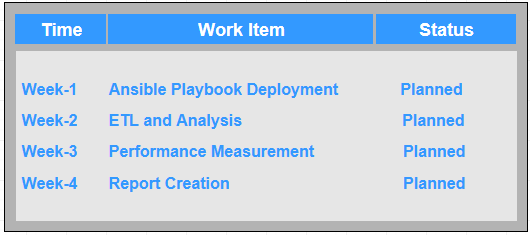
\includegraphics[scale=0.6]{images/image11}
\caption{Planned Schedule}
\end{figure}

\section{Design}

I break the high-level design of the technologies used into 3 main sections-- storage, ingestion, processing and analyzing. 

\begin{itemize}
  \item Storage refers to decision around the storage system such as HDFS or HBase ~\cite{wiki-hadoop}
  \item Ingestion refers to getting data from source and loading it into Hadoop for processing.
  \item Analyzing refers to running various analytical queries on processed dataset to find answer and insight to the questions presented. 
\end{itemize}



\section{Dataset Metadata Description}

The columns included in the dataset download from Kaggle ~\cite{www-kaggle} site  are followed  : 

\begin{itemize}
 \item  \verb|CASE_STATUS|: Status associated with the last significant event or decision.
 \item \verb|EMPLOYER_NAME|: Name of employer submitting labor condition application.
 \item  \verb|SOC_NAME|: the occupational code associated with the job being requested for temporary labor condition, as classified by the Standard Occupational Classification (SOC) System.
 \item  \verb|JOB_TITLE|: Title of the job
 \item  \verb|FULL_TIME_POSITION|: Y = Full Time Position; N = Part Time Position
 \item  \verb|PREVAILING_WAGE|: Prevailing Wage for the job being requested for temporary labor condition. The wage is listed at annual scale in USD. The prevailing wage for a job position is defined as the average wage paid to similarly employed workers in the requested occupation in the area of intended employment. The prevailing wage is based on the employer’s minimum requirements for the position. 
 YEAR: Year in which the H-1B visa petition was filed
 \item  WORKSITE: City and State information of the foreign worker's intended area of employment
 \item  LON: longitude of the Worksite
 \item  LAT: latitude of the Worksite
\end{itemize}

\section{Deployment}
Solution will be deployed using Ansible \cite{wiki-ansible} ad-hoc commands and Linux commands. Driver script called \verb|cc_main_driver.sh|  should install all necessary software and project codes to the cluster nodes.  The \verb|cc_main_driver.sh|  will copy both Python script \verb|called cc_analyze_data.py| which analyzes and generates graphs/tables and shell script \verb| called cc_etl_data.sh| into clusters. The \verb|cc_main_driver.sh|  will trigger \verb|cc_etl_data.sh| to pull dataset from the web as well executes \verb|cc_analyze_data.py| to analyze a dataset. 

\begin{figure}[H]
 \centering
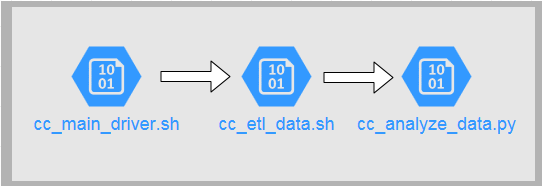
\includegraphics[scale=0.6]{images/image22}
\caption{Deployment Schema}
\end{figure}

\section{Benchmarking}
 The original input dataset with approximately 3,000,000 rows \verb|(h1b_3mRows)| split into two smaller datasets: 1,000,000 rows \verb|(h1b_1mRows)| rows and 2,000,000 rows \verb|(h1b_2mRows)|. Then, I  executed Python script with Linux time function ( i.e:  \verb|time python ./cc_analyze_data.py|)  against each of the input dataset mentioned above in order to measure both the storage size and elapsed time during the execution. 
 
 The benchmark testing on Chameleon Cloud environment revealed in the Figure-4 that elapsed processing time decreased  when the number of rows in the dataset reduced. In the Figure-5, similar trend applied to disk space usage that it decreased linearly  as  the less number of rows need to be stored.


\begin{figure}[H]
  \centering
  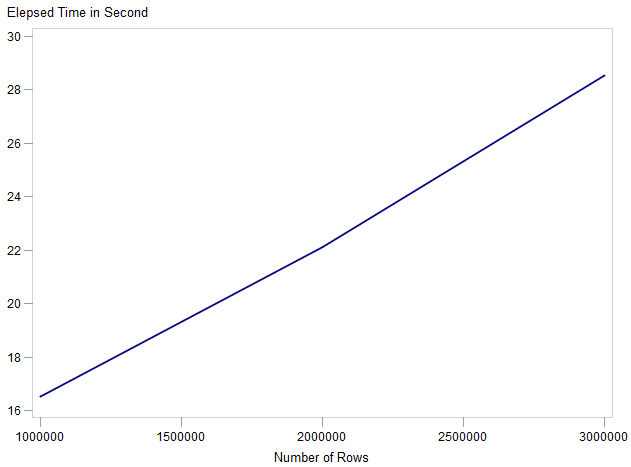
\includegraphics[width=0.5\textwidth]{images/image21}     
  \caption{Benchmark Testing - Number of Rows Vs. Elapsed Time}
  \end{figure}
  
  \begin{figure}[H]
  \centering
  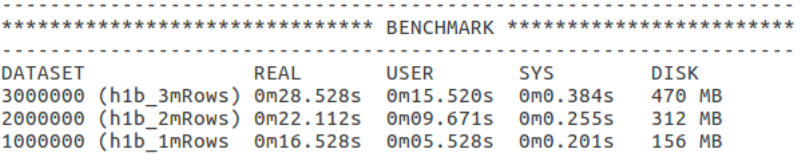
\includegraphics[width=0.5\textwidth]{images/image20}     
  \caption{Benchmark Testing - Number of Rows Vs. Disk Storage }
  \end{figure}


\section{ Data Report}

General  petition distribution between Fiscal Year(FY) 2011 to FY 2016, United States Citizenship and Immigration Services (USCIS) approved 2,615,623 petitions submitted  by the employer on behalf of alien workers as indicated in the Figure-5.  

Of the petitions approved during FY 2011-2016, a total 10,132 petitions, or \verb|.38 %|  were  Data Science related occupations (i.e:  Data Scientist, Data Analytics, Data Science Engineer, Statistician and Data Modelling) as shows in the Figure-6. 

\begin{figure}[H]
  \centering
  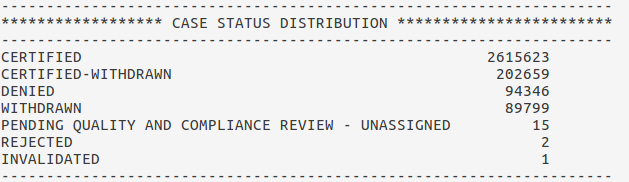
\includegraphics[width=0.5\textwidth]{images/image14} 
  \caption{General Distribution of Petition  - All Jobs}
  \end{figure}

\begin{figure}[H]
  \centering
  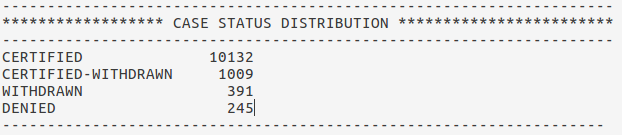
\includegraphics[width=0.5\textwidth]{images/image17}     
  \caption{General Distribution of Petition  - Data Science Related Occupations}
  \end{figure}


As Figure-7 indicated, petitions submitted regardless of the \verb|CASE_STATUS| and all \verb|JOB_TITLE| increased approximately 5 to 7 percent. For Data Science related petitions also increased especially in metropolitan areas such as San Francisco, New York and Menlo Park . The highest number of petition related to Data Science petitions to acquire H1-B visa was in the Fiscal Year 2016 as shown on the Figure-8.

\begin{figure}[H]
  \centering
  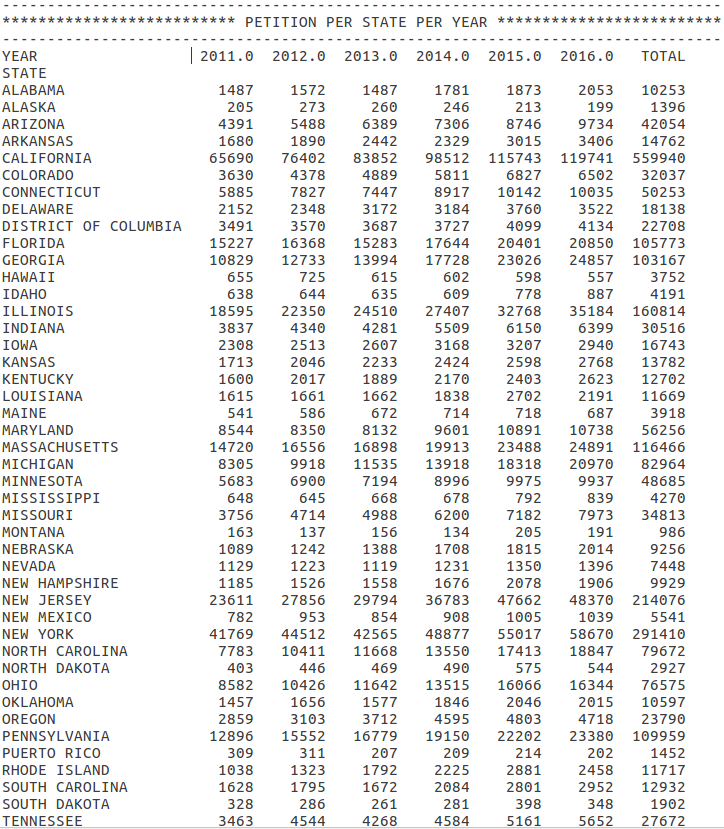
\includegraphics[width=0.5\textwidth]{images/image13} 
       \vspace{-1em}
  \caption{H1-B Petition Per Year Per State - All Jobs}
       \vspace{-1em}
  \end{figure}

\begin{figure}[H]
  \centering
  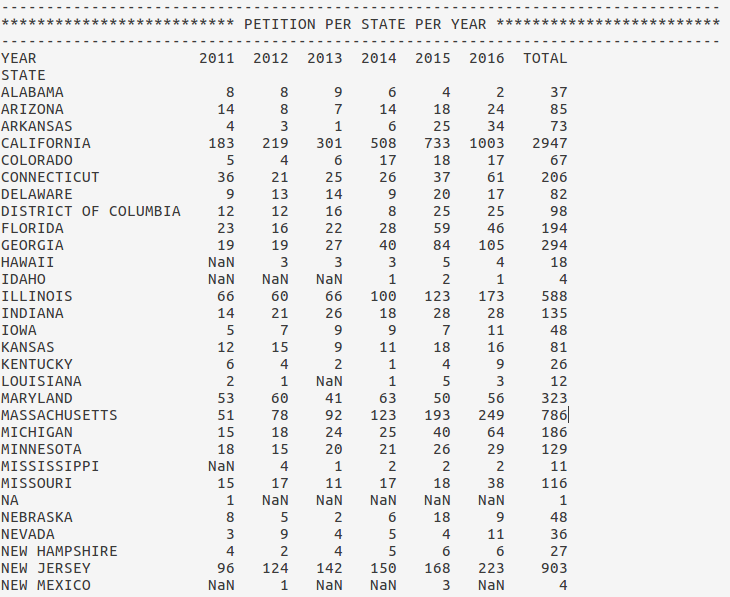
\includegraphics[width=0.5\textwidth]{images/image18}
     \vspace{-1em}
  \caption{H1-B Petition Per Year Per State - Data Science Related Occupations}
     \vspace{-1em}
  \end{figure}

As revealed in Figure-9, New Jersey, California, Massachusetts and Illinois are top locations that hires Data Science talents. Almost all technology based companies are now aware that data-driven decision making is critical if they want to succeed. As showed in the Figure-10, some of the biggest and well-known technology companies are the biggest driving force in hiring talent pool with Data Science skills. 

\begin{figure}[H]
  \centering
  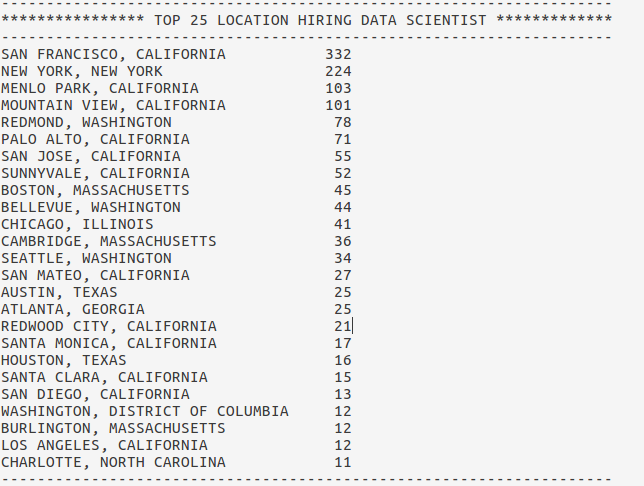
\includegraphics[width=0.5\textwidth]{images/image12}  
   \vspace{-1em}
  \caption{Top 25 Location Hiring Data Scientist}
   \vspace{-1em}
  \end{figure}

\begin{figure}[H]
  \centering
  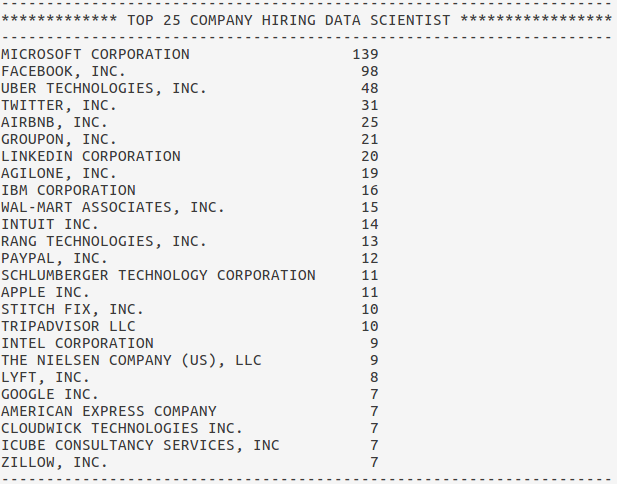
\includegraphics[width=0.5\textwidth]{images/image15}
     \vspace{-1em}
  \caption{Top 25 Companies Hiring Data Scientist}
     \vspace{-1em}
  \end{figure}
  

As shown in Figure-11, for occupations in Data Science field, the median annual compensation reported by employers of H-1B workers  between FY 2011 to FY 2016 was ranged from a low of \verb|$40,000| to  a high \verb|$110,000| which depends on geological location. 

\begin{figure}[H]
  \centering
  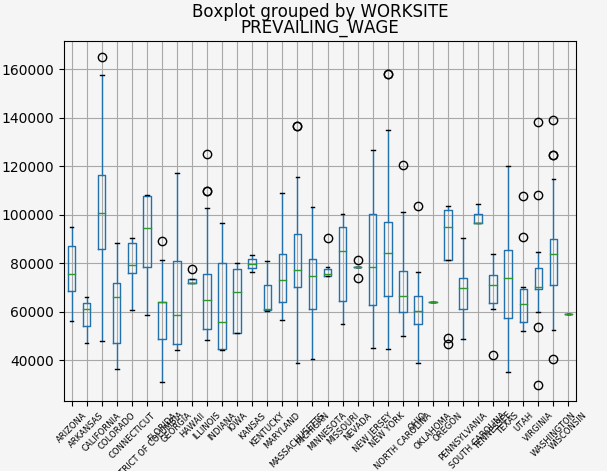
\includegraphics[width=0.5\textwidth]{images/image16} 
    \vspace{-1em}
  \caption{Data Scientist Wage Across States}
    \vspace{-1em}
  \end{figure}


\section{Conclusion}

Overall, there is compelling evidence that the H-1B visa program is helping to alleviate acute shortages in Data Science occupations since the number of petitions submitted increased linearly from FY 2011 to FY 2016.  Armed with such information, as well as indicators presented above, Data Science occupation mostly concentrated in large metropolitan areas. Well-known technology companies has indicated hired professional with Data Science skill sets. 


\section{Acknowledgement}

This work was done as part of the course "I524: Big Data and Open Source Software Projects" at Indiana University during Spring 2017. We acknowledge our Professor Gregor Von Laszewski and all Associate Instructors for helping us and guiding us throughout this project.


% Bibliography

\bibliography{references}
\end{document}

